\section{Software Design}

\subsection{Architecture}

The software on the robot is split between algorythmic and control code that runs on the primary laptop and data aquisition code that runs on the microcontrollers. This allows the laptop to perform all of the intensive calculation allowing the use of very cheap microcontrollers that only need to perform basic low level actions.

The primary language in our system is C++. Object oriented aproaches are used for programs that run on the laptop, while simplified imperitave code is used on the microcontrollers to minimise overhead. Several standard system and computer graphic libraries are used in our code base. The Boost c++ library is used extensivly to provide data structures, serial IO handlers and threads. Image processing is mostly done with algoritms built from elements provided by OpenCV, with some transforms offloaded to the GPU with OpenGL. The codebase currently only runs on linux, however with out migration to Boost we could theoretically port the code base to run on other major platforms (Windows, MacOS, Solaris) with little effort.

\subsection{Algorithms}

\subsubsection{Vision}

The robot uses vision as the primary method of detecting obstacles and lines. The vision algorithm has been developed and modified over several years of competition and is considered reasonably robust. After passing the input video through several different algorithms, a short-term map of the world is created, which the robot is driven off of.

\begin{figure}[H]
\begin{minipage}[b]{0.5\linewidth}
\centering
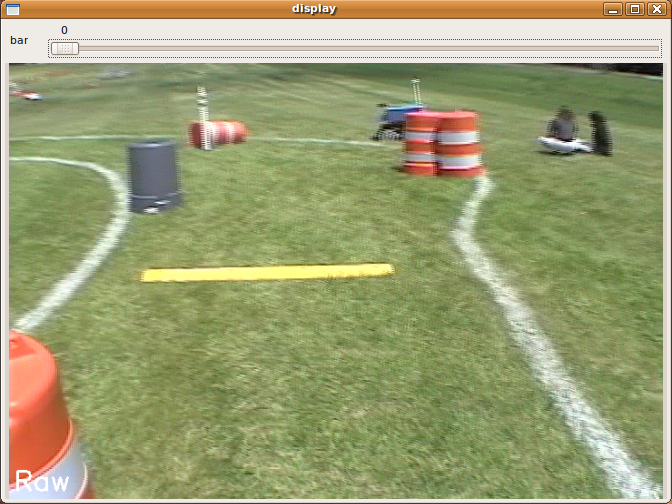
\includegraphics[width=2.5in]{./pics/raw.png}
\caption{Raw Camera Frame}
\label{FIG:Raw}
\end{minipage}
\hspace{0.1in}
\begin{minipage}[b]{0.5\linewidth}
\centering
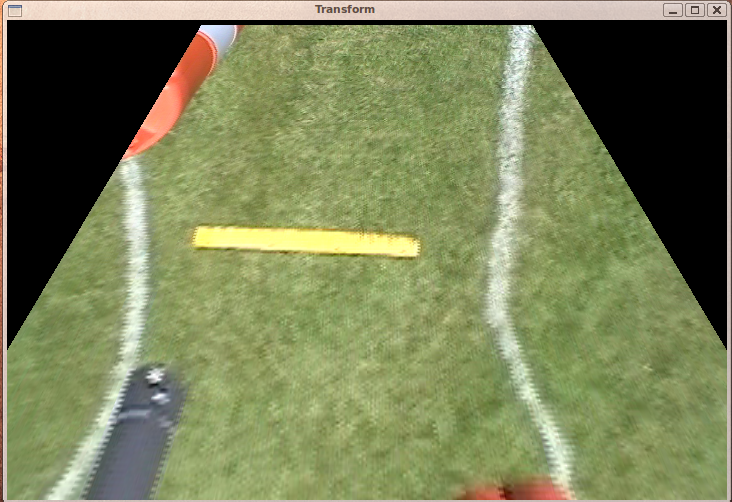
\includegraphics[width=2.5in]{./pics/trans.png}
\caption{Transformed Camera Frame}
\label{FIG:Trans}
\end{minipage}
\end{figure}

The input video, Figure \ref{FIG:Raw}, is first passed through an inverse perspective transform, as seen above-right. This transform makes both near and far off objects a normalized size, and makes the image appear to be taken from directly overhead. This flattened image assumes the course is a plane, which does cause distortion of the barrels, but this is accounted for in the mapping algorithm. The transformed image is much easier to process into a map than a normal, perspective image would be.

The images is then color segmented and thresholded based on the color that is centered directly in front of the robot, as seen above. Safe colors are marked white, the rest are black. The color is averaged in time between frames to allow for some variation in color, for example, if there is dead pach in the grass. This allows the robot to operate on many different surfaces with the same software. For testing we have operated on asphalt parking lots, navigating between the lines marking parking spaces.

\begin{figure}[H]
\begin{center}
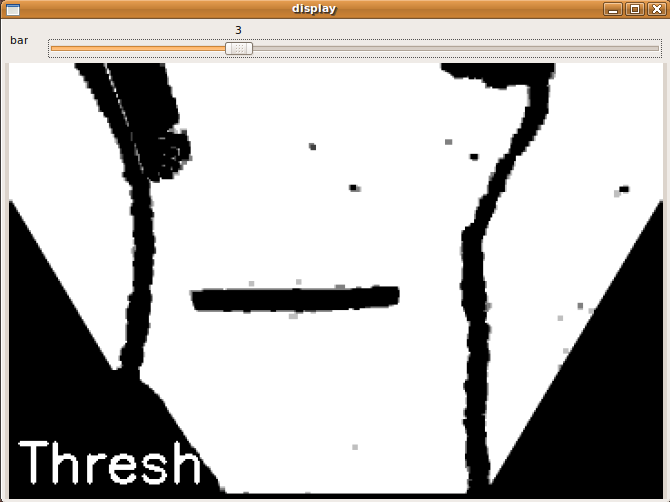
\includegraphics[width=4in]{./pics/thresh.png}
\caption{Color Segmentation Output}
\label{FIG:ColorSeg}
\end{center}
\end{figure}

After converting the transformed image to grayscale, feature tracking is preformed between subsequent frames. The tracked features are denoted by the black lines in the above grayscale image. The algorithm looks for features that have been translated and rotated between frames. This allows us to build a set of likely homographic transform between the images, which can be backed out into likely robot motion between frames. The possible homographic transforms often include several incorrectly matched points, so RANSAC, a nonlinear filter good at outlier handling, is used to reject the outliers and select the best transform.

\begin{figure}[H]
\begin{center}
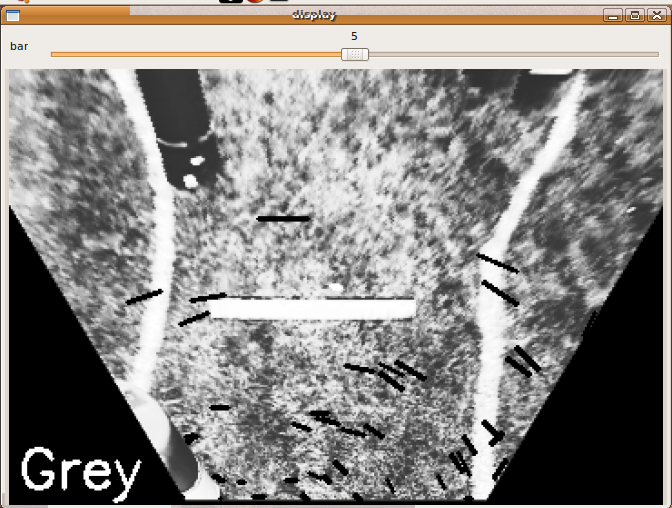
\includegraphics[width=4in]{./pics/feature.png}
\caption{Feature Tracker Output}
\label{FIG:Feature}
\end{center}
\end{figure}

Using motion data, camera frames are drawn into the world map, shown to the right above. The map is a grayscale image, representing a probabilty function of traversablility, where black (0) represents non-traversable, gray (127) represents unknown areas and white(0) represents traversable ares. The map is built up as the robot moves, and slowly decays back to gray to prevent loop closure errors from building up. This map allows the robot to “remember” that it just passed an obstacle and needs to not turn sharply in order to avoid a collision. The robot is driven from the map, by a path planning algorithm.

\begin{figure}[H]
\begin{center}
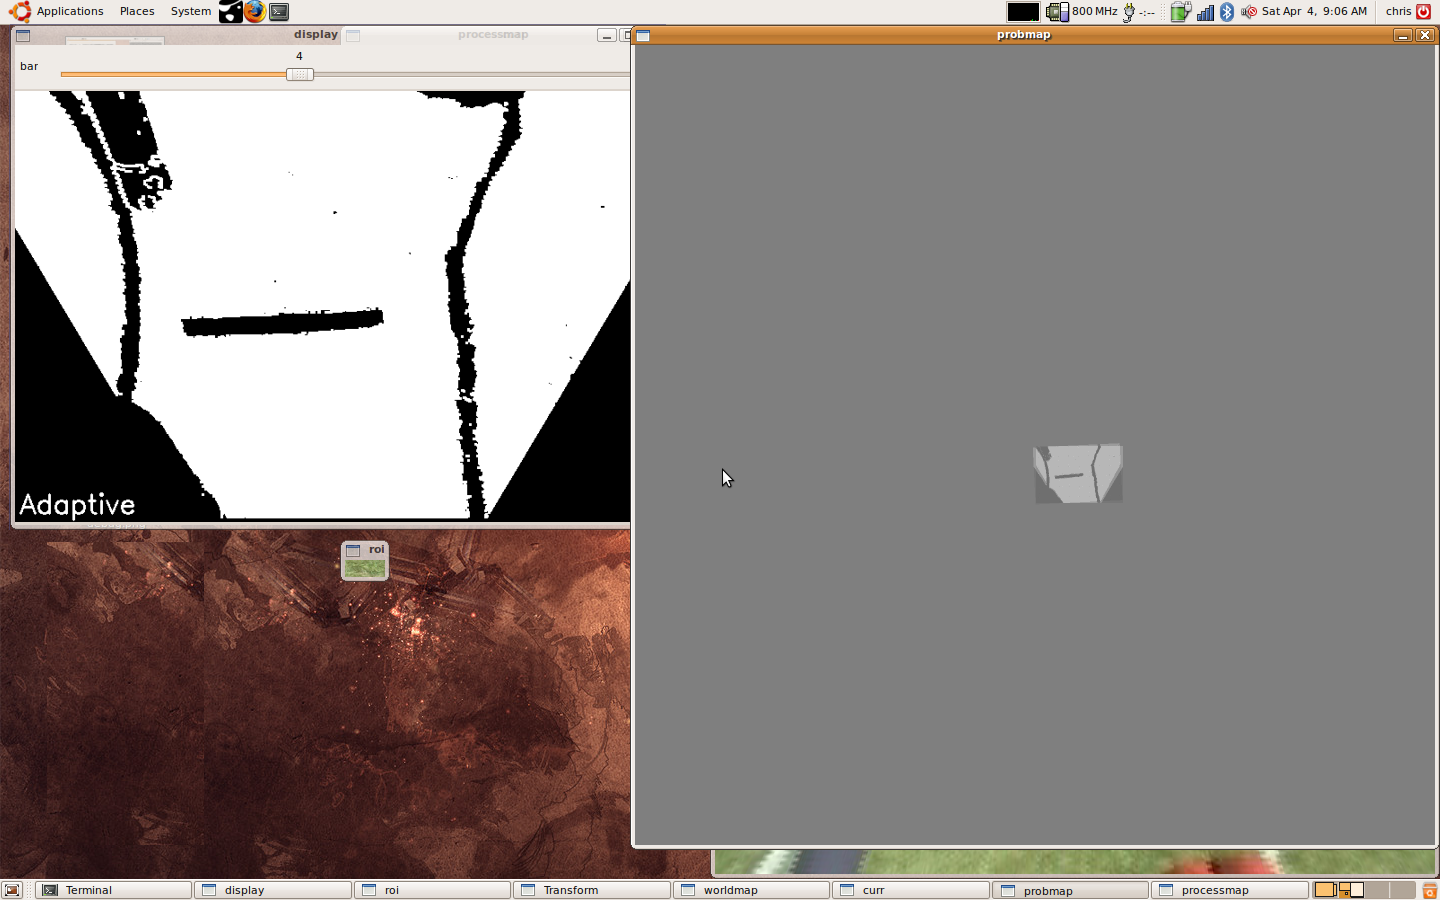
\includegraphics[width=4in]{./pics/map.png}
\caption{World Map}
\label{FIG:Map}
\end{center}
\end{figure}

\subsubsection{Path Planning}

Once the world map is generated, a potential fields algorithm is used. The robot is attracted to the furthest clear point in view and the ramp for the autonmous challenge and the nearest waypoint for the navigation challenge. Obsticals are repel the robot, and the strength of the the field is higher if the object is closer.

\subsubsection{Sensor Filtering}

As our robot has 2 GPS modules, we perform basic filtering to allow the error in the position measurement to be reduced. At this time, a simple average is performed which theoretically reduces random error by a factor of 1.41. We plan to extend this to a full Kalman filter incorperating data from the GPS, wheel encoders, and an IMU (currently not integrated) in future competitions.

\subsubsection{LIDAR}

The LIDAR is used as an obstical and ramp detection sensor. The incoming range information is filtered with a running average to reduce random noise, and is then passed through an erosion-dilation filter to remove islolated points. The $2^{nd}$ derivative is then calculated and thesholded to look for linear objects similar in width to the ramp which when found are given to the path planner as a special goal. Returns with non-zero $2^{nd}$ derivatives are interpreted and given to the path planner as objects to be avoided.
